%% fig_vgmonodromy.tex   (generated by make_round41.py; do not edit by hand)
%% Monodromy of the curves D_a and the Hodge classes of the very general member (lem:vgmonodromy, thm:vgvandermonde).
\documentclass[tikz,border=8pt]{standalone}
\usepackage{amsmath,amssymb}
\usetikzlibrary{arrows.meta,calc,decorations.pathreplacing}
%% palette.tex -- shared colour definitions for the figures
\definecolor{PInk}{RGB}{26,32,44}
\definecolor{PBlue}{RGB}{37,82,139}
\definecolor{PTeal}{RGB}{23,127,125}
\definecolor{POchre}{RGB}{193,138,44}
\definecolor{PClay}{RGB}{178,74,58}
\definecolor{PSlate}{RGB}{108,122,137}
\definecolor{PViolet}{RGB}{110,86,150}
\definecolor{WBlue}{RGB}{223,234,246}
\definecolor{WTeal}{RGB}{220,238,236}
\definecolor{WOchre}{RGB}{250,240,218}
\definecolor{WClay}{RGB}{247,229,224}
\definecolor{WSlate}{RGB}{238,241,244}
\definecolor{PMag}{RGB}{158,58,110}
\definecolor{PGrass}{RGB}{62,124,66}
\definecolor{PAmber}{RGB}{214,112,38}
\definecolor{PIndigo}{RGB}{58,64,140}
\definecolor{PRule}{RGB}{176,186,197}

%% shared macros so the standalone figures match the paper
\providecommand{\QQ}{\mathbb{Q}}
\providecommand{\ZZ}{\mathbb{Z}}
\providecommand{\RR}{\mathbb{R}}
\providecommand{\CC}{\mathbb{C}}
\providecommand{\PP}{\mathbb{P}}
\providecommand{\Kx}{K^{\times}}
\providecommand{\HW}{W}
\providecommand{\Nm}{\mathrm{N}}
\providecommand{\Hdg}{\mathrm{Hdg}}
\providecommand{\NS}{\mathrm{NS}}
\providecommand{\cA}{\mathcal{A}}
\providecommand{\cD}{\mathcal{D}}
\providecommand{\cF}{\mathcal{F}}
\providecommand{\cP}{\mathcal{P}}
\providecommand{\cO}{\mathcal{O}}
\providecommand{\cQ}{\mathcal{Q}}
\providecommand{\bbar}[1]{\overline{#1}}
\providecommand{\ch}{\operatorname{ch}}
\providecommand{\End}{\mathrm{End}}
\providecommand{\Ext}{\operatorname{Ext}}
\providecommand{\Supp}{\operatorname{Supp}}

\begin{document}
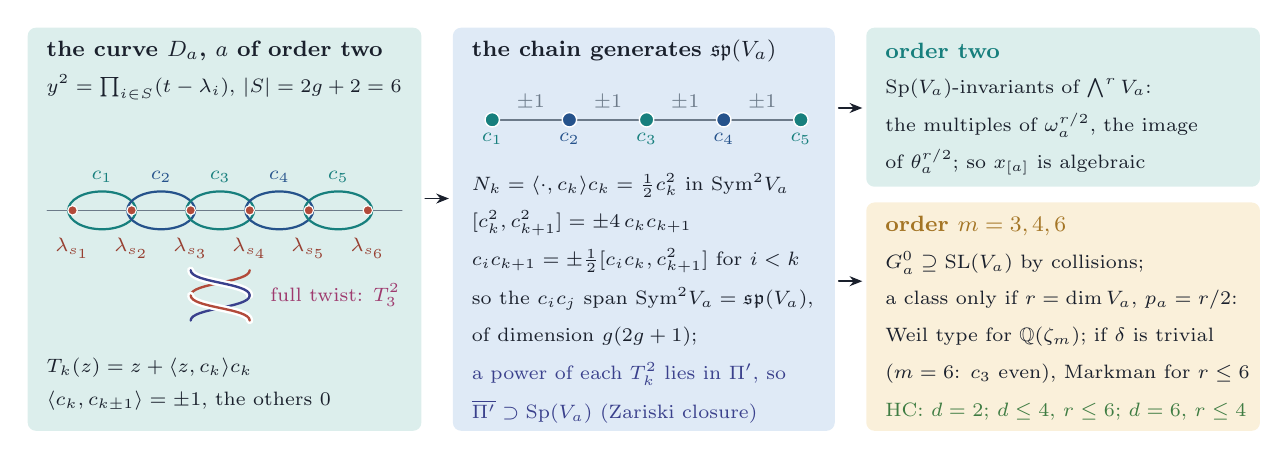
\begin{tikzpicture}[x=1cm,y=1cm,line join=round,line cap=round,
  font=\small,text=PInk,lbl/.style={inner sep=1pt}]
  \path[fill=WTeal,draw=none,rounded corners=3.0pt] (0.0500,-0.5000) rectangle (5.0500,4.6200);
  \path[fill=WBlue,draw=none,rounded corners=3.0pt] (5.4500,-0.5000) rectangle (10.3000,4.6200);
  \path[fill=WTeal,draw=none,rounded corners=3.0pt] (10.7000,2.6000) rectangle (15.7000,4.6200);
  \path[fill=WOchre,draw=none,rounded corners=3.0pt] (10.7000,-0.5000) rectangle (15.7000,2.4000);
  \draw[PSlate,line width=0.6pt] (0.3000,2.3000) -- (4.8000,2.3000);
  \draw[PTeal,line width=0.8pt] (0.9950,2.3000) ellipse (0.4300cm and 0.2400cm);
  \draw[PBlue,line width=0.8pt] (1.7450,2.3000) ellipse (0.4300cm and 0.2400cm);
  \draw[PTeal,line width=0.8pt] (2.4950,2.3000) ellipse (0.4300cm and 0.2400cm);
  \draw[PBlue,line width=0.8pt] (3.2450,2.3000) ellipse (0.4300cm and 0.2400cm);
  \draw[PTeal,line width=0.8pt] (3.9950,2.3000) ellipse (0.4300cm and 0.2400cm);
  \path[fill=PClay,draw=white,line width=0.40pt] (0.6200,2.3000) circle (1.70pt);
  \path[fill=PClay,draw=white,line width=0.40pt] (1.3700,2.3000) circle (1.70pt);
  \path[fill=PClay,draw=white,line width=0.40pt] (2.1200,2.3000) circle (1.70pt);
  \path[fill=PClay,draw=white,line width=0.40pt] (2.8700,2.3000) circle (1.70pt);
  \path[fill=PClay,draw=white,line width=0.40pt] (3.6200,2.3000) circle (1.70pt);
  \path[fill=PClay,draw=white,line width=0.40pt] (4.3700,2.3000) circle (1.70pt);
  \draw[PClay,line width=0.85pt] (2.8700,1.5400) .. controls (2.8700,1.3800) and (2.1200,1.3800) .. (2.1200,1.2200);
  \draw[white,line width=2.6pt] (2.1200,1.5400) .. controls (2.1200,1.3800) and (2.8700,1.3800) .. (2.8700,1.2200);
  \draw[PIndigo,line width=0.85pt] (2.1200,1.5400) .. controls (2.1200,1.3800) and (2.8700,1.3800) .. (2.8700,1.2200);
  \draw[PIndigo,line width=0.85pt] (2.8700,1.2200) .. controls (2.8700,1.0600) and (2.1200,1.0600) .. (2.1200,0.9000);
  \draw[white,line width=2.6pt] (2.1200,1.2200) .. controls (2.1200,1.0600) and (2.8700,1.0600) .. (2.8700,0.9000);
  \draw[PClay,line width=0.85pt] (2.1200,1.2200) .. controls (2.1200,1.0600) and (2.8700,1.0600) .. (2.8700,0.9000);
  \draw[PSlate,line width=0.7pt] (6.0400,3.4500) -- (6.8400,3.4500);
  \draw[PSlate,line width=0.7pt] (7.0200,3.4500) -- (7.8200,3.4500);
  \draw[PSlate,line width=0.7pt] (8.0000,3.4500) -- (8.8000,3.4500);
  \draw[PSlate,line width=0.7pt] (8.9800,3.4500) -- (9.7800,3.4500);
  \path[fill=PTeal,draw=white,line width=0.50pt] (5.9500,3.4500) circle (2.60pt);
  \path[fill=PBlue,draw=white,line width=0.50pt] (6.9300,3.4500) circle (2.60pt);
  \path[fill=PTeal,draw=white,line width=0.50pt] (7.9100,3.4500) circle (2.60pt);
  \path[fill=PBlue,draw=white,line width=0.50pt] (8.8900,3.4500) circle (2.60pt);
  \path[fill=PTeal,draw=white,line width=0.50pt] (9.8700,3.4500) circle (2.60pt);
  \draw[PInk,line width=0.6pt,-{Stealth[length=4.6pt,width=3.6pt]}] (5.1000,2.4500) -- (5.4000,2.4500);
  \draw[PInk,line width=0.6pt,-{Stealth[length=4.6pt,width=3.6pt]}] (10.3500,3.6000) -- (10.6500,3.6000);
  \draw[PInk,line width=0.6pt,-{Stealth[length=4.6pt,width=3.6pt]}] (10.3500,1.4000) -- (10.6500,1.4000);
  \node[lbl,anchor=west,text=PInk,font=\footnotesize] at (0.2500,4.3200) {\textbf{the curve $D_{a}$, $a$ of order two}};
  \node[lbl,anchor=west,text=PInk,font=\scriptsize] at (0.2500,3.8600) {$y^{2}=\prod_{i\in S}(t-\lambda_{i})$, $|S|=2g+2=6$};
  \node[lbl,anchor=south,text=PTeal,font=\scriptsize] at (0.9950,2.6100) {$c_{1}$};
  \node[lbl,anchor=south,text=PBlue,font=\scriptsize] at (1.7450,2.6100) {$c_{2}$};
  \node[lbl,anchor=south,text=PTeal,font=\scriptsize] at (2.4950,2.6100) {$c_{3}$};
  \node[lbl,anchor=south,text=PBlue,font=\scriptsize] at (3.2450,2.6100) {$c_{4}$};
  \node[lbl,anchor=south,text=PTeal,font=\scriptsize] at (3.9950,2.6100) {$c_{5}$};
  \node[lbl,anchor=north,text=PClay!85!black,font=\scriptsize] at (0.6200,1.9900) {$\lambda_{s_{1}}$};
  \node[lbl,anchor=north,text=PClay!85!black,font=\scriptsize] at (1.3700,1.9900) {$\lambda_{s_{2}}$};
  \node[lbl,anchor=north,text=PClay!85!black,font=\scriptsize] at (2.1200,1.9900) {$\lambda_{s_{3}}$};
  \node[lbl,anchor=north,text=PClay!85!black,font=\scriptsize] at (2.8700,1.9900) {$\lambda_{s_{4}}$};
  \node[lbl,anchor=north,text=PClay!85!black,font=\scriptsize] at (3.6200,1.9900) {$\lambda_{s_{5}}$};
  \node[lbl,anchor=north,text=PClay!85!black,font=\scriptsize] at (4.3700,1.9900) {$\lambda_{s_{6}}$};
  \node[lbl,anchor=west,text=PMag,font=\scriptsize] at (3.0900,1.2200) {full twist: $T_{3}^{2}$};
  \node[lbl,anchor=west,text=PInk,font=\scriptsize] at (0.2500,0.3000) {$T_{k}(z)=z+\langle z,c_{k}\rangle c_{k}$};
  \node[lbl,anchor=west,text=PInk,font=\scriptsize] at (0.2500,-0.1200) {$\langle c_{k},c_{k\pm1}\rangle=\pm1$, the others $0$};
  \node[lbl,anchor=west,text=PInk,font=\footnotesize] at (5.6500,4.3200) {\textbf{the chain generates $\mathfrak{sp}(V_{a})$}};
  \node[lbl,anchor=south,text=PSlate,font=\scriptsize] at (6.4400,3.5300) {$\pm1$};
  \node[lbl,anchor=south,text=PSlate,font=\scriptsize] at (7.4200,3.5300) {$\pm1$};
  \node[lbl,anchor=south,text=PSlate,font=\scriptsize] at (8.4000,3.5300) {$\pm1$};
  \node[lbl,anchor=south,text=PSlate,font=\scriptsize] at (9.3800,3.5300) {$\pm1$};
  \node[lbl,anchor=north,text=PTeal,font=\scriptsize] at (5.9500,3.3200) {$c_{1}$};
  \node[lbl,anchor=north,text=PBlue,font=\scriptsize] at (6.9300,3.3200) {$c_{2}$};
  \node[lbl,anchor=north,text=PTeal,font=\scriptsize] at (7.9100,3.3200) {$c_{3}$};
  \node[lbl,anchor=north,text=PBlue,font=\scriptsize] at (8.8900,3.3200) {$c_{4}$};
  \node[lbl,anchor=north,text=PTeal,font=\scriptsize] at (9.8700,3.3200) {$c_{5}$};
  \node[lbl,anchor=west,text=PInk,font=\scriptsize] at (5.6500,2.6200) {$N_{k}=\langle\cdot,c_{k}\rangle c_{k}=\tfrac12c_{k}^{2}$ in $\mathrm{Sym}^{2}V_{a}$};
  \node[lbl,anchor=west,text=PInk,font=\scriptsize] at (5.6500,2.1400) {$[c_{k}^{2},c_{k+1}^{2}]=\pm4\,c_{k}c_{k+1}$};
  \node[lbl,anchor=west,text=PInk,font=\scriptsize] at (5.6500,1.6600) {$c_{i}c_{k+1}=\pm\tfrac12[c_{i}c_{k},c_{k+1}^{2}]$ for $i<k$};
  \node[lbl,anchor=west,text=PInk,font=\scriptsize] at (5.6500,1.1800) {so the $c_{i}c_{j}$ span $\mathrm{Sym}^{2}V_{a}=\mathfrak{sp}(V_{a})$,};
  \node[lbl,anchor=west,text=PInk,font=\scriptsize] at (5.6500,0.7000) {of dimension $g(2g+1)$;};
  \node[lbl,anchor=west,text=PIndigo,font=\scriptsize] at (5.6500,0.2200) {a power of each $T_{k}^{2}$ lies in $\Pi'$, so};
  \node[lbl,anchor=west,text=PIndigo,font=\scriptsize] at (5.6500,-0.2600) {$\overline{\Pi'}\supset\mathrm{Sp}(V_{a})$ (Zariski closure)};
  \node[lbl,anchor=west,text=PTeal,font=\footnotesize] at (10.9000,4.3200) {\textbf{order two}};
  \node[lbl,anchor=west,text=PInk,font=\scriptsize] at (10.9000,3.8500) {$\mathrm{Sp}(V_{a})$-invariants of $\bigwedge^{r}V_{a}$:};
  \node[lbl,anchor=west,text=PInk,font=\scriptsize] at (10.9000,3.3800) {the multiples of $\omega_{a}^{r/2}$, the image};
  \node[lbl,anchor=west,text=PInk,font=\scriptsize] at (10.9000,2.9100) {of $\theta_{a}^{r/2}$; so $x_{[a]}$ is algebraic};
  \node[lbl,anchor=west,text=POchre!85!black,font=\footnotesize] at (10.9000,2.1000) {\textbf{order $m=3,4,6$}};
  \node[lbl,anchor=west,text=PInk,font=\scriptsize] at (10.9000,1.6300) {$G_{a}^{0}\supseteq\mathrm{SL}(V_{a})$ by collisions;};
  \node[lbl,anchor=west,text=PInk,font=\scriptsize] at (10.9000,1.1600) {a class only if $r=\dim V_{a}$, $p_{a}=r/2$:};
  \node[lbl,anchor=west,text=PInk,font=\scriptsize] at (10.9000,0.6900) {Weil type for $\QQ(\zeta_{m})$; if $\delta$ is trivial};
  \node[lbl,anchor=west,text=PInk,font=\scriptsize] at (10.9000,0.2200) {($m=6$: $c_{3}$ even), Markman for $r\le6$};
  \node[lbl,anchor=west,text=PGrass,font=\scriptsize] at (10.9000,-0.2600) {HC: $d=2$; $d\le4$, $r\le6$; $d=6$, $r\le4$};
\end{tikzpicture}
\end{document}
